

\newpage
\chapter{Contactos semiconductor-semiconductor}


\section{Potencial relativo}

Tomando el silicio intrínseco como referencia, se puede calcular el potencial relativo sin tensión aplicada mediante la regla de los 60 mV de un trozo de silicio dopado. La regla establece que por cada orden de magnitud de dopado se incrementa su potencial relativo al silicio intrínseco por 60mV. El potencial relativo para el caso de electrones es: 

\[ V_{n} = V_{T} \ln \left(\dfrac{n_{b}}{10^{10}} \right) = 60\ mV \log \left(\dfrac{n_{b}}{10^{10}}\right) \]

Donde $n_{b}$ es la concentración de electrones o de huecos respecto a la cual se requiere calcular el potencial relativo. Para material tipo N implica un potencial positivo y para material tipo P implica un potencial negativo.

Por otro lado el potencial relativo para el caso de huecos, está dado por:

\[ V_{n} = -60\ mV \log \left(\dfrac{p_{b}}{10^{10}}\right) \]

Donde $p_{b}$ es la concentración de huecos o electrones respecto a la cual se requiere calcular el potencial relativo. Para material tipo P implica un potencial positivo y para material tipo N implica un potencial negativo.

Debido a que la corriente neta debe de ser nula, la diferencia de potencial se requiere para que la corriente de difusión cancele a la corriente de arrastre.

\newpage
\section{La unión PN}

La unión de un bloque de silicio P con un bloque de silicio N da como resultado el siguiente diagrama de bandas:

\begin{figure}[H]
    \centering
    \includegraphics[width=0.8\textwidth]{figuras/union-pn_despues.pdf}
    \caption{Diagrama de bandas de una unión PN, después del doblamiento de bandas.}
    \label{union-pn_despues}
\end{figure}


\newpage
\subsection{Potencial de contacto}

\[ V_{bi} = \dfrac{kT}{q} \ln \dfrac{N_A N_D}{n_i^2} \]





\subsection{Ley de la juntura}

En ambos lados de la juntura existe una concentración definida de electrones y huecos. La concentración de a ambos lados es:

\[ \phi_p = V_T \ln \dfrac{n_p}{n_i} \] 

\[ \phi_n = V_T \ln \dfrac{n_n}{n_i} \]

Restando ambos potenciales:

\[ \phi_B = \phi_n - \phi_p \]

\[ \phi_B = V_T \ln \dfrac{n_n}{n_i} - V_T \ln \dfrac{n_p}{n_i} \]

\[ \phi_B = V_T \ln \left( \dfrac{n_n n_i}{n_i n_p} \right) \]

\[ \phi_B = V_T \ln \left( \dfrac{n_n}{n_p} \right) \]

De esta última expresión se puede despejar la concentración de electrones del lado p:

\[ n_p = n_n e^{-\phi_B/V_T} \]

Y sabiendo que la concentración de electrones en el lado n es aproximadamente igual a la concentración de átomos donadores:

\[ \boxed{n_p = N_D e^{-\phi_B/V_T}} \]

El análisis se repite con la concentración de huecos, de manera que se obtiene:

\[ p_n = p_p e^{-\phi_B/V_T} \]

\[ \boxed{p_n = N_A e^{-\phi_B/V_T}} \]

Estas últimas cuatro ecuaciones son conocidas  como la Ley de la Juntura: \textbf{la concentración de portadores minoritarios de un lado de la unión depende de la concentración de portadores mayoritarios del otro lado y de un factor exponencial.}

\subsection{Ancho de la zona de agotamiento}

El ancho de la región de agotamiento es:

\[ x_n = \sqrt{\dfrac{2 \epsilon_0 \epsilon_r N_A V_{bi}}{q N_D (N_A + N_D)}} \]

\[ x_p = \sqrt{\dfrac{2 \epsilon_0 \epsilon_r N_D V_{bi}}{q N_A (N_A + N_D)}} \]

\[ x_B = x_n + x_p = \sqrt{\dfrac{2 \epsilon_0 \epsilon_r N_D V_{bi}}{q} \left( \dfrac{1}{N_A} + \dfrac{1}{N_D} \right)} \]

\subsection{Capacitancia en equilibrio}

La capacitancia en equilibrio es:

\[ C_{j0} = \sqrt{\dfrac{\epsilon_0 \epsilon_r q}{2} \dfrac{N_A N_D}{N_A + N_D} \dfrac{1}{V_{bi}} } \]


\subsection{Capacitancia de reversa}

\[ C_j = \dfrac{C_{j0}}{\sqrt{1 - \dfrac{V_R}{V_bi}}} \]


\subsection{Capacitancia de directa}

La capacitancia de directa es función del tiempo de tránsito de los portadores, y de la corriente que fluye a través del diodo:

\[ C_d = \dfrac{\tau_T}{V_T} I_D \]

%\textbf{Problema 4.2.} Considere el gráfico dado en la Figura \ref{fig-CapacidadInversa.pdf}, que corresponde a la capacidad en inversa de una unión \textit{pn}, expresada por unidad de área. Considere además que la unión tiene un área transversal de 2000 $\mu$m$^2$ y que la tensión térmica es de 26 mV.

%\begin{figure}[H]
%    \centering
%    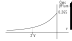
\includegraphics[width=0.8\textwidth]{figuras/CapacidadInversa.pdf}
%    \caption{Capacidad de unión en polarización inversa}
%    \label{fig-CapacidadInversa.pdf}
%\end{figure}

%Determine: 

%\begin{itemize}
%\item La capacidad de la unión en 0 V de tensión aplicada.
%\item El nivel de dopado $N_a$ y $N_d$, sabiendo que $N_{a}/N_{d}=$2.22 y el potencial en $x_{n}$ es de 0.3573V.
%\item El potencial de contacto de la unión PN.
%\item La capacidad de la unión en -2 V de tensión aplicada.
%\item La longitud de la zona de vaciamiento del lado N ($x_{p}$).
%\item La longitud de toda la zona de vaciamiento ($x_{B}$).
%\item El diagrama de bandas del dispositivo en estado de equilibrio térmico, mostrando la deformación de bandas e indicando los niveles de $E_C$, $E_V$, $E_i$, $E_F$, $x_{n}$ y $x_{p}$.
%\end{itemize}
